% !TEX root = catron-dissertation.tex
\epstopdfsetup{outdir=./images/03_aero_optics_acoustics/}

\chapter{Aero-Optical and Acoustical Coupling}
\label{chap:03_optical_acoustics}

% \begin{itemize}
%   \color{red}
%   \item
% \end{itemize}

Acoustic waves are isentropic compression waves with the fluctuating pressure, $p'$, determining the strength of the wave.
This fluctuating pressure is related to the sound pressure level, $\spl$ by
\begin{equation}
  \spl = 20\log_{10}\left(\frac{p_{RMS}}{p_0}\right)
  \label{eqn:03_spl}
\end{equation}
where $p_{RMS}$ is the root mean square of the pressure fluctuation, and $p_0$ is the reference pressure (20 $\mu$Pa for air).
The pressure fluctuations can be related to the density fluctuations via the definition of the speed of sound:
\begin{equation}
  c_0^2 = \left(\frac{\partial p}{\partial \rho}\right)_s=\frac{p'}{\rho'}
  \label{eqn:03_speed_sound}
\end{equation}
where $c_0$ is the speed of sound at mean fluid properties and the subscript $s$ denotes constant entropy.
It can be shown by combining Equations \ref{eqn:02_gladstone_dale_relation_fluctuating} and \ref{eqn:02_opd} that the fluctuating density can be related to the $\opd$,
\begin{equation}
  \opd = K_{GD}\int_{s_1}^{s_2}{\rho'}ds \textrm{.}
  \label{eqn:03_opd_fluct}
\end{equation}
This can be combined with Equation \ref{eqn:03_speed_sound},
\begin{equation}
  \opd = \frac{K_{GD}}{c_0^2}\int_{s_1}^{s_2}{p'}ds \textrm{,}
  \label{eqn:03_opd_pressure}
\end{equation}
to provide a way of computing the optical path difference of a sound pressure field.

\section{Simulating an Optical Wavefront Measurement from an Acoustic Field Function}
\label{sect:03_simulated_beam}
The following analysis is presented for the case of a measurement field subject to acoustic excitation at a discrete frequency. Parameter values at each point in the field oscillate at the frequency of the acoustic field, with a magnitude and phase relationship to the acoustic field that can be represented by complex notation and that depends on the physics of the interaction with the acoustic field.

The effect of a complex acoustic pressure field on an optical wavefront can be simulated by applying Equation \ref{eqn:03_opd_pressure}.
To accomplish this, two separate coordinate systems will need to be defined.
The first is the beam coordinate system, $\mathbf{x}_B $, that will have a measurement aperture, which is typically circular, defined in the xy-plane and assuming the beam propagates in the z-direction.
The second is the acoustic coordinate system, $\mathbf{x}_A$, that will be defined based on the source location or the geometry that the acoustic waves are propagating through.
A function representing the transformation from one coordinate system to the other can be defined as
\begin{equation}
  \mathbf{x}_A = R\mathbf{x}_B+T \textrm{,}
  \label{eqn:03_coord_transform}
\end{equation}
where $R$ is a matrix which represents the rotation and $T$ is a vector that represents the translation.

The important parameters for defining the aperture on which the beam coordinate system is based are the aperture size, $Ap$, and the spatial discretization which, if the beam is measured using a Shack-Hartmann wavefront sensor, is the number of lenslets or sub-apertures in the wavefront sensor, $N_{lenslets}$.
Assuming that the aperture is either circular or square and the lenslet size and sub-aperture size is approximately $Ap/N_{lenslets}$, the x locations of the center of the sub-apertures go from $-Ap/2(1-1/N_{lenslets})$ to $Ap/2(1-1/N_{lenslets})$ by steps of $Ap/N_{lenslets}$ with the y locations having the same values.
This gives a matrix representing both $x_{Ap}$ and $y_{Ap}$ that is $N_{lenslets}$ by $N_{lenslets}$.
For the purpose of removing piston, tip, and tilt and creating a mask that represents the beam aperture, the radial coordinates, $\rho_{Ap}$ and $\theta_{Ap}$, of the aperture should also be calculated.
A circular beam will have a mask defined by,
\begin{equation}
  Mask_{Ap} =
  \begin{cases}
    1, & \text{if } \rho_{Ap}\leq Ap/2 \\
    0, & \text{otherwise.}
  \end{cases}
\end{equation}
The beam coordinate frame is the aperture coordinates extruded in the z-direction over the range of desired z-values.

After the beam coordinates are transformed into the acoustic coordinates using Equation \ref{eqn:03_coord_transform}, the complex pressure field, $\hat{p}(x,y,z,t)$ can be calculated at the points that are within the optical beam.
If the pressure field is separable into spatial and temporal components, then the integration along the beam length only needs to be done once for each temporal frequency,
\begin{equation}
  \widehat{\opd}(x,y) = \frac{K_{GD}}{c_0^2}\int_{z_1}^{z_2} \hat{p}(x,y,z)_{Ap}dz \textrm{,}
  \label{eqn:03_opd_complex}
\end{equation}
where $\widehat{\opd}(x,y)$ is the complex optical path difference as measured in the aperture plane.
If a complex density field is known instead, than Equation \ref{eqn:03_opd_complex} becomes
\begin{equation}
  \widehat{\opd}(x,y) = K_{GD}\int_{z_1}^{z_2} \hat{\rho}(x,y,z)_{Ap}dz \textrm{.}
  \label{eqn:03_opd_complex_density}
\end{equation}
For the purposes of calculating time-averaged optical properties of simulated beam passing through a known complex pressure or density field a phase vector was defined,  $\phi = [0, 2\pi)$.
The measurable component as a function of phase is
\begin{equation}
  \opd(x,y,\phi) = \real\left[\widehat{\opd}(x,y)\exp\{-j\phi\}\right] \textrm{,}
  \label{eqn:03_opd_real_phase}
\end{equation}
or as a function of time for all temporal frequencies,
\begin{equation}
  \opd(x,y,t) = \real\left[\sum\widehat{\opd}(x,y)\exp\{-j\omega t\}\right] \textrm{,}
  \label{eqn:03_opd_real}
\end{equation}
where there is a separate $\widehat{\opd}(x,y)$ computed for each temporal frequency.
One of the more important parameters that can be calculated from $\opd$ is the spatial RMS, $\opdrms$, which is calculated at each time or phase step at the points where the aperture mask equals one.

\section{Simple Examples of Acoustic-Optical Coupling}
\label{sect:03_examples}
Two basic acoustic pressure fields will be numerically examined for their optical properties.
The first will be a planar acoustic wave that will be numerically simulated over a variety of conditions.
The second will be a spherical acoustic wave that will be both numerically simulated and validated experimentally.

\subsection{Planar Acoustic Waves}
\label{sect:03_examples_planar}
A planar wave is the simplest solution to the wave equation and varies only in time and the direction of travel.
A planar wave can be calculated from the set of solutions for duct acoustics, Equation \ref{eqn:02_pressure_solution_duct}, given that $\Psi_m(x,y)=1$,
\begin{equation}
  \hat{p}(z,t) = C_m\exp\left\{j(\omega t \mp k_{zm}^\pm z)\right\} \textrm{.}
  \label{eqn:03_plane_wave}
\end{equation}
This section will show the effect that acoustic waves have on the optical wavefront of a planar wave with the general geometry shown in Figure \ref{fig:03_planar_sample_domain}.
\begin{figure}
  \centering
  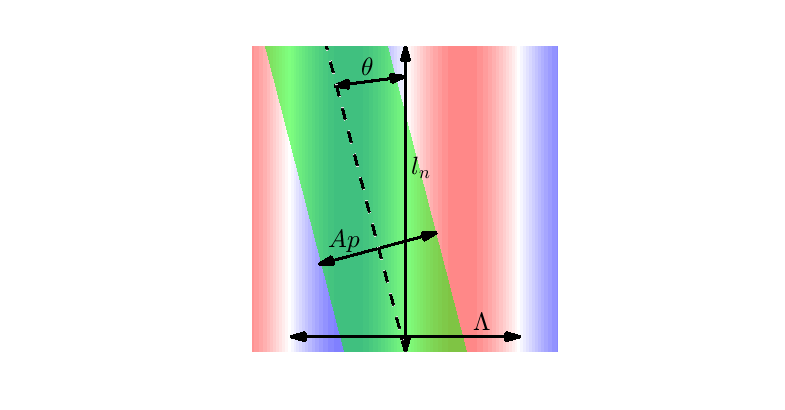
\includegraphics{../matlab/03_aero_optics_acoustics/planar_sample_domain.eps}
  \caption{General geometry for various sample calculations for showing the acoustic-optical coupling effect.}
  \label{fig:03_planar_sample_domain}
\end{figure}
For the following example, $l_n$ is the width of the acoustic disturbance (for example, the width of the wind tunnel), $\theta$ is the angle between the planar acoustic wave and the beam direction, $A_p$ is the aperture diameter of the beam, and $\Lambda$ is the wavelength of the acoustic wave.

Figure \ref{fig:03_planar_sample_calc_3} shows the time averaged $\opdrms$ per meter of beam propagation when the beam path is parallel ($\theta=0$) to the peaks and troughs of the planar acoustic wave as $\spl$ is varied.
\begin{figure}
  \centering
  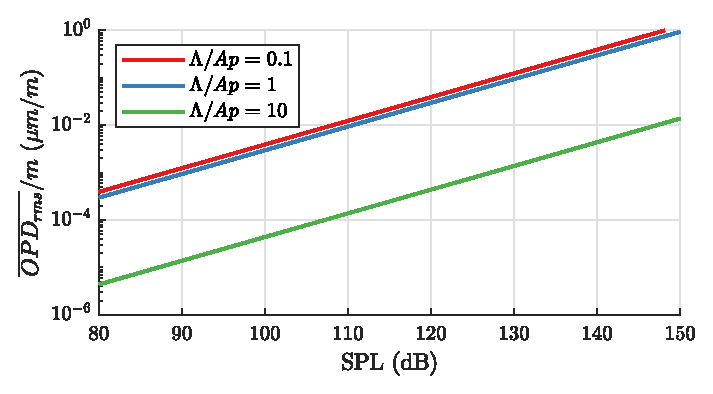
\includegraphics{../matlab/03_aero_optics_acoustics/planar_sample_calc_3.eps}
  \caption{Theoretical time-averaged $\opdrms$ per meter of beam propagation as a function of sound pressure level, $\spl$, for several $\Lambda/Ap$ ratios and $\theta=0$.}
  \label{fig:03_planar_sample_calc_3}
\end{figure}
As the sound pressure level increases the time averaged $\opdrms$ also increases and can easily reach the point of being a significant factor in the measured optical disturbance.
There is little difference between 0.1 and 1 $\Lambda/Ap$, but as the wavelength gets much larger compared to the beam diameter, then the optical effect of the noise is greatly reduced, this effect is known as ``aperture filtering.''
Aperture filtering accounts for the fact that an aperture that is smaller than the wavelength of the optical disturbance only passes a portion of that optical disturbance, so that the measured $\opdrms$ is reduced \cite{Siegenthaler-2005-KQ2HGmfp}.

The effect of aperture filtering is more clearly shown in Figure \ref{fig:03_planar_sample_calc_1}.
\begin{figure}
  \centering
  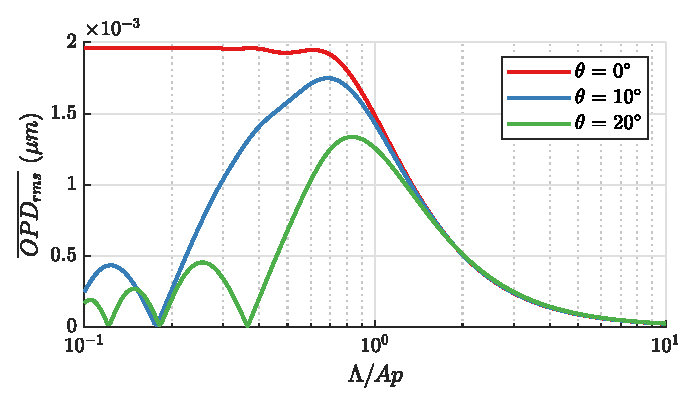
\includegraphics{../matlab/03_aero_optics_acoustics/planar_sample_calc_1.eps}
  \caption{Theoretical time-averaged $\opdrms$ for a RMS sound pressure of 1 Pa ($\spl$ of 94 dB), $l_n$ of 1 m, and various angles and $\Lambda/Ap$ ratios.}
  \label{fig:03_planar_sample_calc_1}
\end{figure}
As the $\Lambda/Ap$ ratio increases from 0.1, time-averaged $\opdrms$ remains fairly constant until it starts to drop around $\Lambda/Ap$ of 0.7 and starts to asymptotically approach zero which it basically reaches by $\Lambda/Ap$ of 10.
Figure \ref{fig:03_planar_sample_calc_1} also shows the effect of changing the beam angle, $\theta$, through the acoustic field.
For nonzero $\theta$, the beam encounters alternating high and low index of refraction as it passes through the test region, so that the time-averaged $\opdrms$ begins to decrease compared to the $\theta = 0^\circ$ case below $\Lambda/Ap=1$.
There are also points of zero optical disturbance that occur at $\theta_{zero}=\tan^{-1}(n\Lambda/l_n)$ for $n\neq0$; these points occur because the peaks and valleys of the optical disturbance caused by the sound wave effectively cancel out over the length of the integration path, $l_n/\cos\theta$.

Figures \ref{fig:03_planar_sample_calc_3} and \ref{fig:03_planar_sample_calc_1} show the optical effect of plane acoustic waves in a no-flow environment.
The effect of wind-tunnel flow is to stretch (downstream-traveling waves) or compress (upstream-traveling waves) the wavelength of the acoustic noise thereby altering the filtering effect of the beam aperture.
Figure \ref{fig:03_planar_sample_calc_2} shows a typical optical disturbance from the two transverse acoustic waves (u+c and u-c) present in a wind tunnel at Mach 0.6.
\begin{figure}
  \centering
  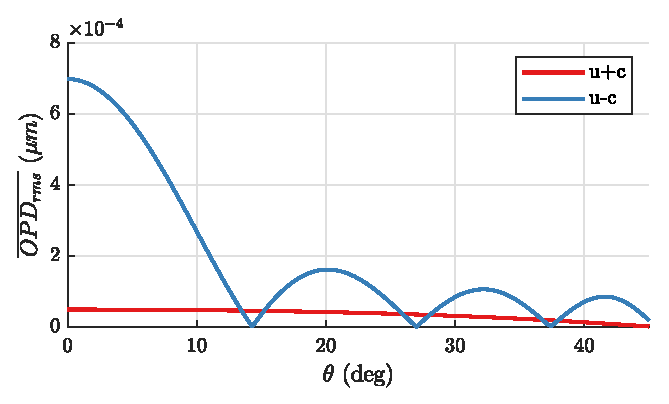
\includegraphics{../matlab/03_aero_optics_acoustics/planar_sample_calc_2.eps}
  \caption{Theoretical time-averaged $\opdrms$ for the two acoustic waves (u+c and u-c) for the blade pass frequency (534 Hz) at Mach 0.6 with a RMS sound pressure of 1 Pa ($\spl$ of 94 dB), $l_n$ of 1 m, and $Ap$ of 15 cm.}
  \label{fig:03_planar_sample_calc_2}
\end{figure}
Both waves have an RMS sound pressure of 1 Pa and the beam has an aperture of 15 cm and propagates through an acoustic field inside a duct of width, $l_n$, of 1 m.
Over the vast majority of the look back angles the upstream-traveling acoustic wave has a much greater effect on the optical disturbance compared to the downstream-traveling acoustic wave, due to the much shorter wavelength of the upstream-traveling waves which is less affected by aperture filtering.
However, the upstream-traveling wave goes through several zero points so that the downstream-traveling wave dominates at some beam angles.

% In summary, Figures \ref{fig:03_planar_sample_calc_3} to \ref{fig:03_planar_sample_calc_2} give an example of how planar acoustic waves are expected to affect a beam traveling a finite distance $l_n$ at an angle $\theta$ through the acoustic field.

\subsection{Spherical Acoustic Waves}
\label{sect:03_examples_spherical}
The acoustic field from a speaker may be assumed to be a spherical wave from a pulsating point if the frequency is sufficiently low and the measurement region is far enough away from the source \cite{Randall-1951-9NtPPXPq}.
This pressure field when converted to complex pressure is represented by
\begin{equation}
  \hat{p}(r,t) = \frac{A_0}{r}\exp\left\{-j(kr-\omega t)\right\} \textrm{,}
  \label{eqn:03_spherical_pressure}
\end{equation}
where $A_0$ is the fluctuating pressure strength and $r$ is the distance from the source to the measurement point.
The RMS pressure of this field can be represented by
\begin{equation}
  p_{RMS} = \frac{|A_0|}{r\sqrt{2}} \textrm{.}
  \label{eqn:03_spherical_pressure_rms}
\end{equation}

\subsubsection{Theoretical $\opd$ Calculations}
A set of optical properties were calculated for a beam passing through a spherical acoustic field as defined by a point source using the process described previously in Section \ref{sect:03_simulated_beam} and shown in Figure \ref{fig:03_spherical_simulation}.
\begin{figure}
  \centering
  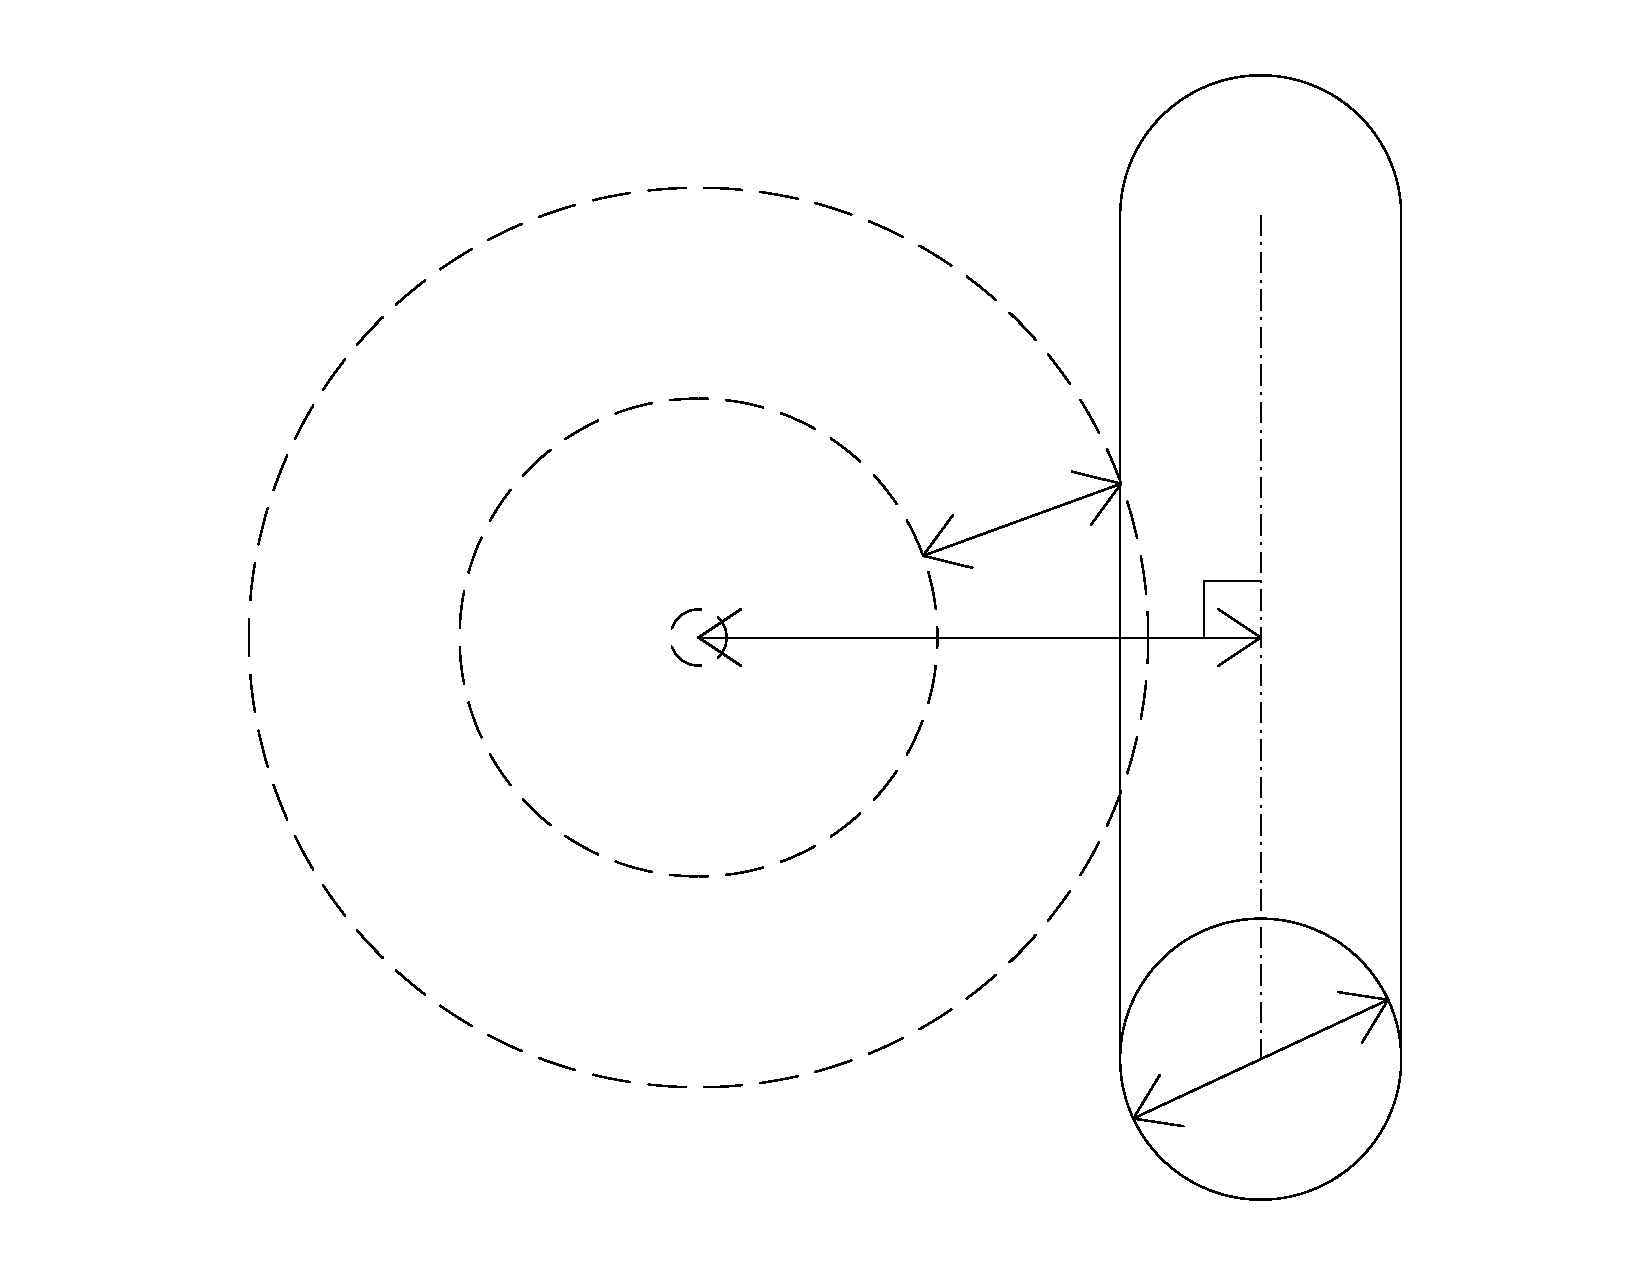
\includegraphics[width=0.8\textwidth]{../cad/spherical_simulation.pdf}
  \put(-140,130){\fcolorbox{white}{white}{\large $R$}}
  \put(-140,155){\fcolorbox{white}{white}{\large $\Lambda$}}
  \put(-95,43){\fcolorbox{white}{white}{\large $Ap$}}
  \put(-240,115){\large Acoustic Source}
  \put(-70,100){\rotatebox{90}{\large Beam}}
  \caption{Diagram of the geometry used in the spherical wave simulation.}
  \label{fig:03_spherical_simulation}
\end{figure}
These calculations used a circular aperture size of 0.25 m in diameter that was assumed to be measured using a Shack-Hartmann WFS with 32x32 sub-apertures with a non-dimensional acoustic wavelength, $\Lambda$, of $Ap/4$ to $10Ap$.
The normal vector from the point source to the axis of the measurement beam defined the coordinate system.
This normal distance, $R$, was a minimum $5Ap$ and a maximum of $25Ap$, keeping the measurement beam away from the singularity at the origin of the acoustic source.
The $\opd$ for the beam was integrated over a distance of $\pm5$-m from the plane of the point source.
To calculate the time-averaged $\opdrms$ the phase of the source was varied from 0 to $2\pi$ with 25 total steps.

The result of these $\opdrms$ calculations is shown in Figure \ref{fig:03_spherical_sample}.
\begin{figure}
  \centering
  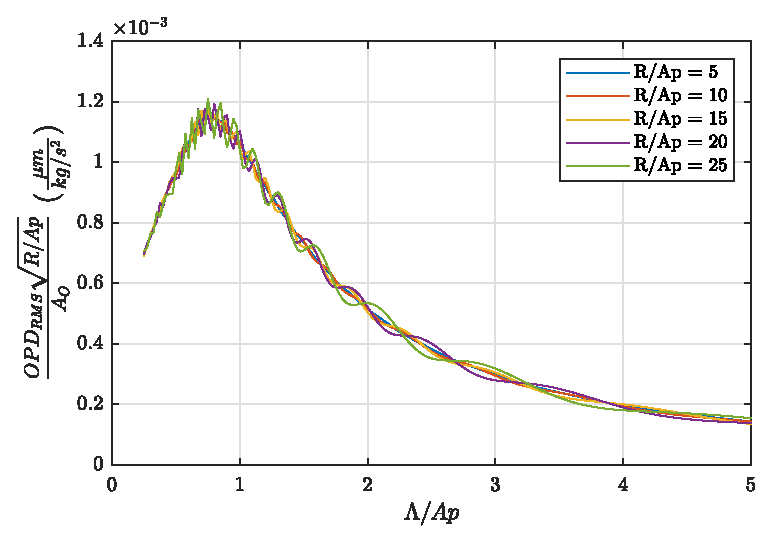
\includegraphics{../matlab/03_aero_optics_acoustics/spherical_sample.eps}
  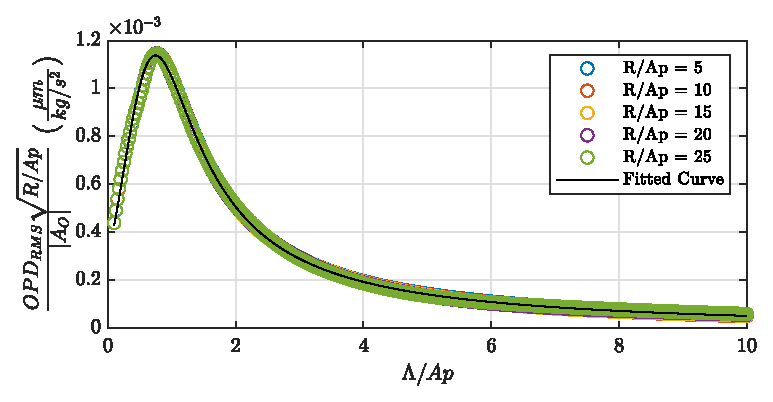
\includegraphics{../matlab/03_aero_optics_acoustics/spherical_sample_win.eps}
  \caption{Theoretical time-averaged $\opdrms$ for a spherical acoustic wave. The top plot shows a perfect spherical acoustic signal integrated over $\pm$5 m. The bottom plot shows has a Tukey window applied along the beam length to partially emulate source directivity which significantly reduces the measured oscillations.}
  \label{fig:03_spherical_sample}
\end{figure}
The top plots shows the expected optical disturbance ratio, $\opdrms/|A_0|$, for a perfectly spherical acoustic field measured over the beam length.
The oscillations in the solutions for different $R/Ap$ are caused by end effects in the integration.
Because speakers often have a directivity in their emission, the oscillations can be greatly reduced by using a windowing function in the z-direction, such as a Hanning \cite{Oppenheim-1999-cfwyTmwq},
\begin{equation}
  w(x) = \frac{1}{2}\left\{1-\cos\left(2\pi x\right)\right\} \textrm{,}
\end{equation}
or Tukey window \cite{Bloomfield-2000-vD9dkPMd},
\begin{equation}
  w(x) = \begin{cases}
    \frac{1}{2}\left\{1+\cos\left(\frac{2\pi}{r}\left[x-\frac{r}{2}\right]\right)\right\}, & 0\leq x < \frac{r}{2} \\
    1, & \frac{r}{2}\leq x < 1-\frac{r}{2} \\
    \frac{1}{2}\left\{1+\cos\left(\frac{2\pi}{r}\left[x-1+\frac{r}{2}\right]\right)\right\}, & 1-\frac{r}{2} \leq x \leq 1
  \end{cases}
\end{equation}
the roughly model this directivity as shown in the bottom plot.
While this plot was calculated with a single aperture diameter, the general trend holds for all other aperture diameters that were tested, the only effect was the size and width of the oscillations.

The peak of the optical disturbance ratio, $\opdrms/|A_0|$, is located at $\Lambda/Ap\approx0.75$ for a circular aperture.
The signal is reduced above this value due to aperture filtering and below this value because the shorter wavelengths have a reduced distance before alternating high and low index-of-refraction regions reduce the optical path difference.
When the acoustic source point is sufficiently far enough away from the measurement beam, $R/Ap\geq2$, the optical disturbance ratio, $\opdrms/|A_0|$ when multiplied by $\sqrt{R/Ap}$, can be collapsed onto a single curve for a range of $\Lambda/Ap$ of 0.1 to 10.
Above $\Lambda/Ap=10$ the curves start to diverge away from one another.
An approximate function fit to these data is
\begin{equation}
  \frac{\opdrms\sqrt{R/Ap}}{|A_0|} \approx \frac{p_1(\Lambda/Ap)^3+p_2(\Lambda/Ap)^2+p_3(\Lambda/Ap)+p_4}{(\Lambda/Ap)^3+q_1(\Lambda/Ap)^2+q_2(\Lambda/Ap)+q_3}
  \label{eqn:03_spherical_sample_fit}
\end{equation}
with coefficient values shown Table \ref{tab:03_spherical_sample_coeff}.
This functional fit has a coefficient of determination, $R^2$, value of 0.9991.
\begin{table}
\centering
\caption{Curve fit values for Figure \ref{fig:03_spherical_sample} and Equation \ref{eqn:03_spherical_sample_fit}}
\input{../matlab/03_aero_optics_acoustics/spherical_sample_win.txt}
\label{tab:03_spherical_sample_coeff}
\end{table}


\subsubsection{Measurement of a Spherical Acoustic Wave with an Optical Beam}
A small bench top experiment was used to compare the simultaneous optical and microphone measurements of an acoustic field from a speaker as shown in Figure \ref{fig:03_speaker_test}.
\begin{figure}
  \centering
  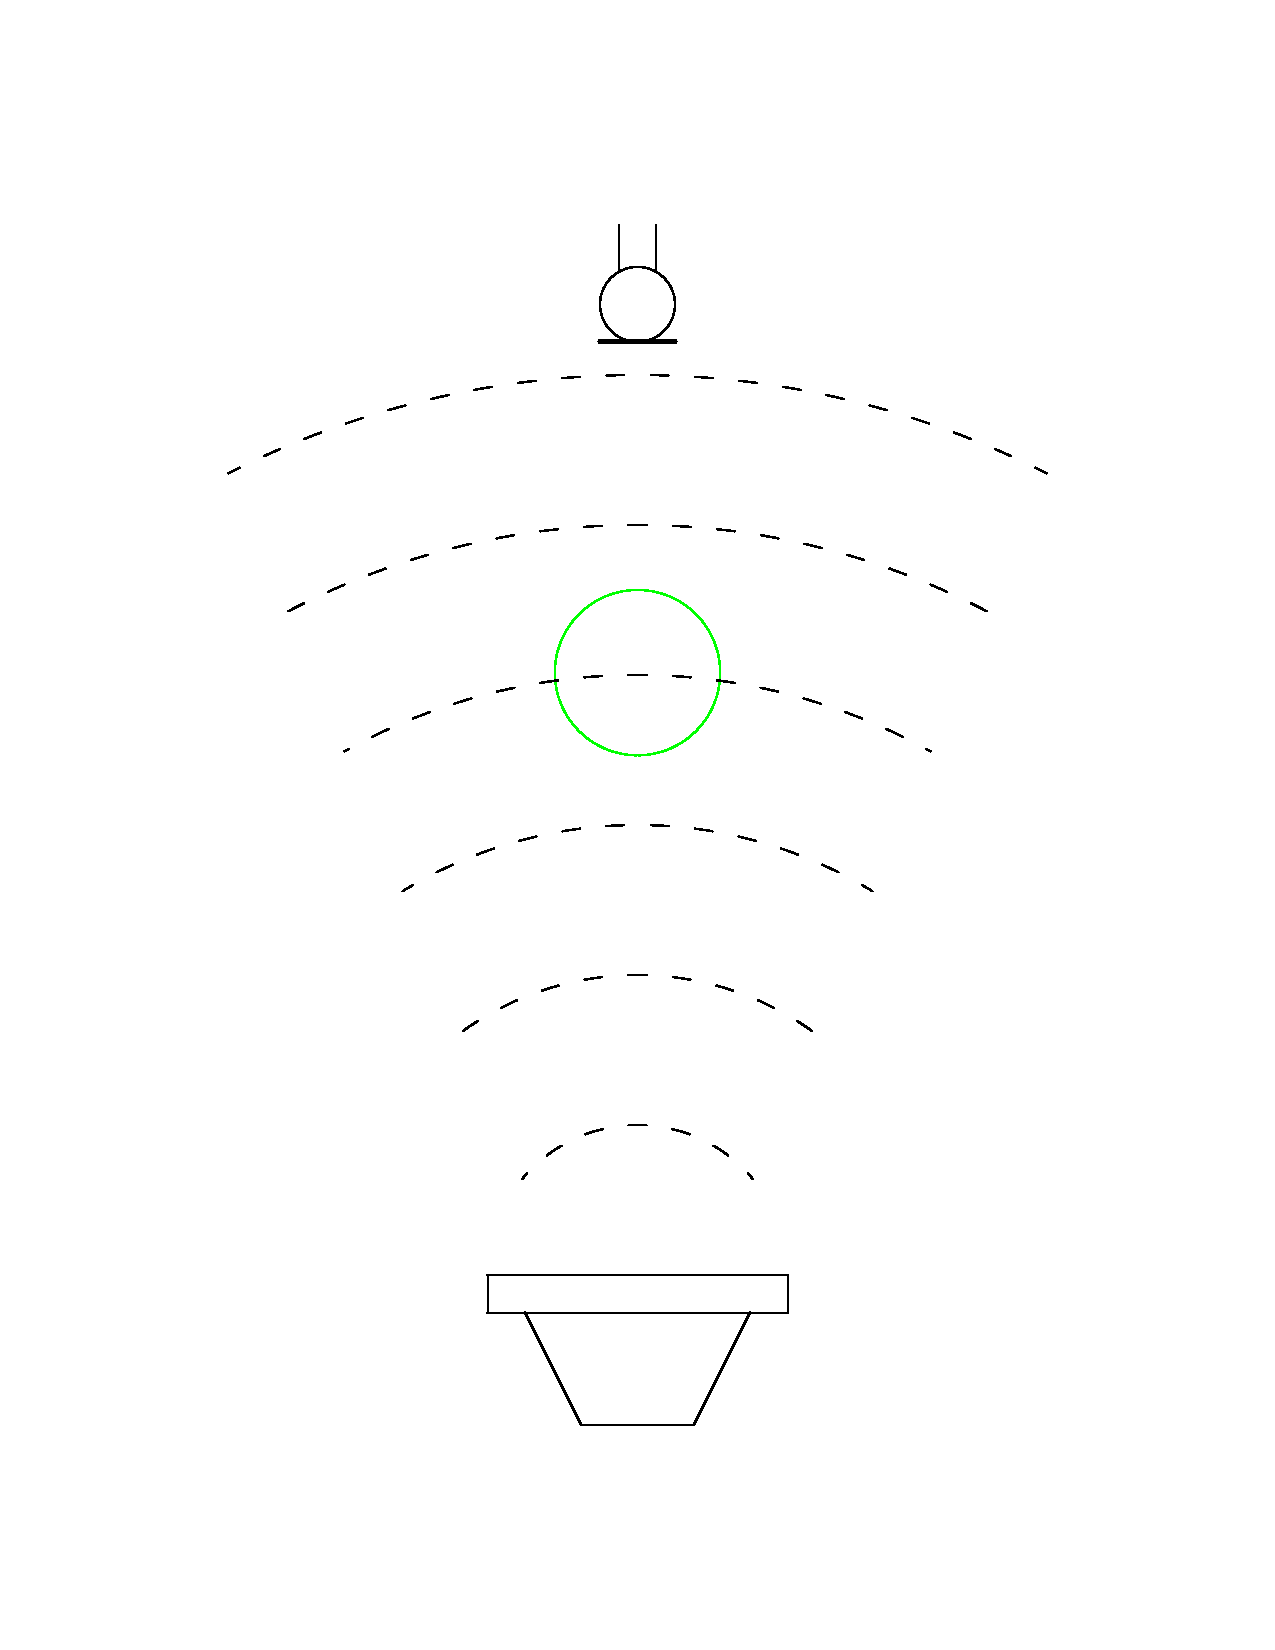
\includegraphics[width=3.5in,clip,trim=100 100 100 100]{../cad/speak_test.pdf}
  \put(-146,25){\large Speaker}
  \put(-141,230){\large Beam}
  \put(-160,310){\fcolorbox{white}{white}{\large Microphone}}
  \caption{Spherical acoustic wave measurement test.}
  \label{fig:03_speaker_test}
\end{figure}
The distance from the center of the beam to the speaker was 102 mm with a beam diameter of 28 mm.
An ACO model 7016B microphone \cite{ACO-Microphones} was placed directly over the speaker at a distance of 158 mm and was used with a Br\"uel \& Kj\ae r model 2670 preamplifier \cite{Bruel-Kjaer-2670}.
The speaker used was a Peerless model XT25SC90-04 \cite{Peerless-XT25SC90-04-1} which has a fairly flat on-axis response from 1 kHz to 40 kHz.
% A Br\"uel \& Kj\ae r model 2690 \cite{Bruel-Kjaer-2690} signal conditioner was used as part of the data aquiztion system

The wavefront measurements system utilized in these measurements is similar to that shown in Figure \ref{fig:02_typical_wavefront_system} except there was no primary telescope.
The speaker was located in the center of the measurement region which was about 2 feet in length and the re-imaging telescope reduced the beam diameter by a factor of two and re-imaged the return mirror.
Optical wavefronts and microphone measurements were taken at 49 kHz.
The speaker was sinusoidally excited at three different frequencies (9, 14, and 18 kHz) at a variety of voltages.

The absolute value of the fluctuating pressure strength, $|A_0|$, was calculated two different ways.
First, the power spectrum of the microphone data was used to calculate the average $p_{RMS}$ at the excitation frequency and the fluctuating pressure strength using Equation \ref{eqn:03_spherical_pressure_rms}.
For the second method, the optical wavefront was band-pass filtered at the excitation frequency using a process that will be discussed in Chapter \ref{chap:06_single_filter}.
The time averaged $\opdrms$ of the filtered wavefront data was then used to calculate the fluctuating pressure strength using Equation \ref{eqn:03_spherical_sample_fit}.

The results of these measurements of the fluctuating pressure strength is shown in Table \ref{tab:03_spherical_measurement}.
The differences between the two techniques for measuring the fluctuating pressure strength fell into two groups.
For the 9 kHz cases, the differences ranged from 20-26\% while for the higher frequency cases the differences were between 1.1-1.5\%.
In all cases the wavefront measurement reported a higher fluctuating pressure strength.
With the exception of the highest excitation case at 9 kHz, the differences between the to techniques was fairly constant for each frequency group.
Some of these differences may be attributable to the frequency response of the microphone.
\begin{table}
  \centering
  \caption{Comparison of microphone and wavefront computation of $|A_0|$}
  \input{../matlab/03_aero_optics_acoustics/spherical_measurement.txt}
  \label{tab:03_spherical_measurement}
\end{table}

In Figure \ref{fig:03_spherical_plot}, measured wavefronts are compared to the wavefronts simulated using the method described in Section \ref{sect:03_simulated_beam} for the highest excitation cases at each frequency.
\begin{figure}
  \centering
  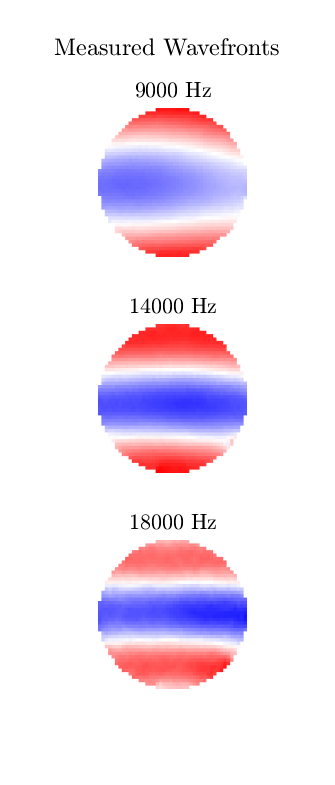
\includegraphics{../matlab/03_aero_optics_acoustics/spherical_plot_measured.eps}
  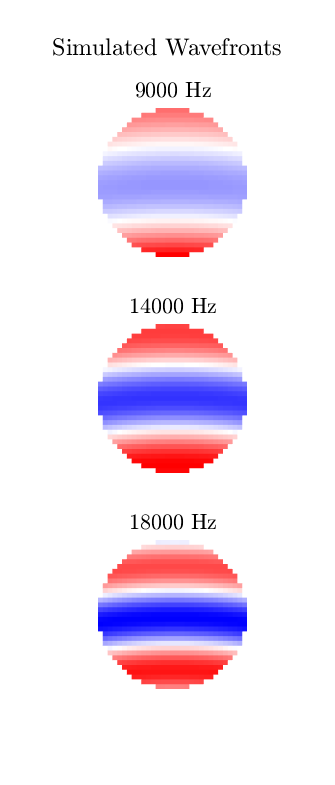
\includegraphics{../matlab/03_aero_optics_acoustics/spherical_plot_simulated.eps}
  \caption{Comparison of measured wavefront to simulated ones for the highest-amplitude speaker excitation at each frequency.}
  \label{fig:03_spherical_plot}
\end{figure}
The 9 kHz case shows some anomalies on the measured wavefront on the right side, and deviates from a spherical wave significantly, likely contributing to the significantly higher estimated pulsating field strength value when compared to the microphone estimate in Table \ref{tab:03_spherical_measurement}.
The 14 and 18 kHz cases show some remarkable agreement between the measured and simulated images.
Optical wavefront measurements can therefore be used for making non-intrusive acoustic field measurements especially when the acoustic field is simple.



\section{Estimating the Acoustic Field Inside a Wind-Tunnel Test-Section}
\label{sect:03_test_section}
Several mode-matching methods have been previously employed to solve the acoustic field in ducts, ranging from methods designed to solve axially-segmented turbofan duct liners \cite{McAlpine-2006-NrCzhW4Z} to muffler modeling \cite{Ji-2013-agaCHhcP}.
These methods require the entire field to be solved simultaneously because there are duct modes traveling in both directions at each axial-spatial location.
Using the turbofan duct liner version, a single azimuthal order, $m$, and only a few radial orders, $n$, need to be computed for the various boundary conditions with a constant mesh used through all the segments.
In the muffler model version, step changes in the cross-section are employed, allowing for a constant mesh to be generated to account for all possible cross-sections.

For a wind-tunnel that has numerous cross-sectional area changes, specifically, a square cross-section for the test-section and a circular cross-section for the fan, the mode-matching method can become computational expensive.
At each axial-location, all possible duct modes need to be calculated up to at the very least the cutoff mode $k_m$, if not higher \cite{Gabard-2008-H4mEEeVt}, to fully resolve local duct modes.
As such, in order to reduce the computational cost of simulating the acoustic environment inside of a wind tunnel, a mode marching method was employed instead of a mode-matching method, where an initial cross-sectional pressure field was marched from the wind-tunnel fan in both directions around the wind-tunnel and through the test-section.
Although the mode-marching method is computationally simpler than the mode-matching method, there are also arguments for using the mode-marching method that are justified by the expected acoustic behavior in typical wind-tunnel circuits.
Specifically, since the wind-tunnel test section normally has the smallest cross-sectional dimensions, higher-order acoustic modes tend to be reflected away from the test section; hence using a mode-marching method that does not rigorously account for reflections or all high-order modes should not add significant inaccuracy to the predicted results.

For the circular to square transition on either side of the wind-tunnel fan, a deformable mesh was used such that there would be a one-to-one mapping of mesh points throughout the transition.
An example of the deformable mesh is shown in Figure \ref{fig:deformable_mesh} at both the square and circular limits and halfway in between.
\begin{figure}
  \centering
  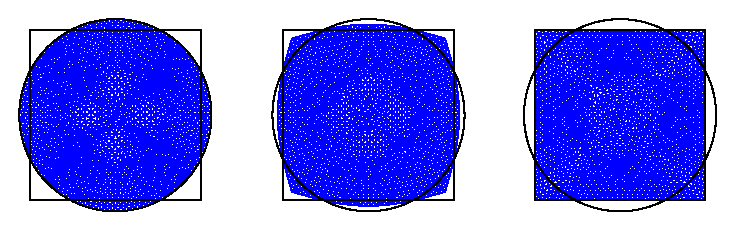
\includegraphics[width=\textwidth]{../matlab/03_aero_optics_acoustics/deformable_mesh.eps}
  \caption{Deformable mesh for calculating the acoustic modes in the circular to square transitions at three stages.}
  \label{fig:deformable_mesh}
\end{figure}
Because cross-sectional wavenumber scales with the area ($k_m^2A=\textrm{const}$), all modes were solved for a cross-section of unit area.
For the simulation of the Notre Dame White Field wind tunnel (described below) modes in the square cross-sections of the wind tunnel were calculated with both the deformable mesh and a rectangular mesh in order to allow for easy transitions in the cruciform region of this wind-tunnel's diffuser.

\subsection{Mode-Marching Method Procedure}
\label{sect:03_test_section_mode_marching}
\begin{enumerate}
  \item \textit{Starting Acoustic Pressure Disturbance} \\
  The method starts with an initial acoustic pressure disturbance that could be either measured, computed, or assumed.
  \begin{equation}
    \hat{p}^0(x,y)
  \end{equation}
  For wind tunnels, the acoustic disturbance is generated by the main fan; hence $\hat{p}^0$ is the rotating radial fan modes associated with the rotating fan blades \cite{Cumpsty-1989-8wEYqb7t}.

  \item \textit{Modal Best Fit} \\
  The pressure disturbance at the current axial location is best fit to the possible modes.
  \begin{equation}
    \hat{p}^i(x,y)=\Psi_m^i(x,y)\cdot C_m^i
  \end{equation}
  where $\Psi_m^i$ are the possible modes for the local duct shape.

  \item \textit{Transmitted Pressure Ratio} \\
  The pressure attenuation due to Mach number change \cite{Powell-1959-W7KVArvn} as a ratio of transmitted pressure to incident pressure is computed for an acoustic wave traveling with subsonic flow,
  \begin{equation}
    \frac{p_t}{p_i} = \left(\frac{1+M_n}{1+M_{n+1}}\right)\left(\frac{2M_{n+1}}{M_n+M_{n+1}}\right)\left(\frac{X_{n,n}}{X_{n,n+1}}\right)\left(\frac{X_{n,n}}{X_{n+1,n+1}}\right)^{1/(\gamma-1)} \textrm{,}
    \label{eqn:03_pressure_ratio_with}
  \end{equation}
  or traveling against subsonic flow,
  \begin{equation}
    \frac{p_t}{p_i} = \left(\frac{1-M_n}{1-M_{n+1}}\right)\left(\frac{2M_{n+1}}{M_n+M_{n+1}}\right)\left(\frac{X_{n,n}}{X_{n,n+1}}\right)\left(\frac{X_{n,n}}{X_{n+1,n+1}}\right)^{1/(\gamma-1)} \textrm{,}
    \label{eqn:03_pressure_ratio_against}
  \end{equation}
  where
  \begin{equation}
    X_{a,b} = 1+\frac{\gamma-1}{2}M_aM_b \textrm{.}
  \end{equation}

  \item \textit{Reflected Pressure Ratio} \\
  The reflected pressure ratio is a useful quantity to keeping track of, because one of the main assumptions of the mode marching method is that the reflections are negligible.
  The pressure attenuation due to Mach number change \cite{Powell-1959-W7KVArvn} as a ratio of reflected pressure to incident pressure is computed for an acoustic wave traveling with subsonic flow,
  \begin{equation}
    \frac{p_r}{p_i} = \left(\frac{1+M_n}{1-M_n}\right)\left(\frac{M_{n+1}-M_n}{M_{n+1}+M_n}\right)\frac{Y_{n,n+1}}{X_{m,n+1}} \textrm{,}
    \label{eqn:03_pressure_ratio_with_reflected}
  \end{equation}
  or traveling against subsonic flow,
  \begin{equation}
    \frac{p_r}{p_i} = \left(\frac{1-M_n}{1+M_n}\right)\left(\frac{M_{n+1}-M_n}{M_{n+1}+M_n}\right)\frac{Y_{n,n+1}}{X_{m,n+1}} \textrm{,}
    \label{eqn:03_pressure_ratio_against_reflected}
  \end{equation}
  where
\begin{equation}
  Y_{a,b} = 1-\frac{\gamma-1}{2}M_aM_b \textrm{.}
\end{equation}

  \item \textit{March Modes Forward} \\
  March the acoustic modes forward to the next axial location.
  \begin{equation}
    \hat{p}_{i+1}(x,y) = \frac{p_t}{p_i}\sum\Psi_M^i(x,y)\cdot C_m^i\cdot\exp\{\mp j k_{zm}^\pm z\}
  \end{equation}

  \item \textit{Repeat} \\
  Repeat steps 2-5 until the desired location is reached (i.e. the wind-tunnel test section).
  Different starting pressure disturbances can also be checked.
\end{enumerate}

\subsection{University of Notre Dame White Field Wind-Tunnel Simulation}
\label{sect:03_test_section_sim}
The University of Notre Dame White Field wind-tunnel is capable of reaching speeds of Mach 0.6 in the 3 foot by 3 foot test-section.
A CAD model of the wind-tunnel is shown in Figure \ref{fig:03_tunnel_model}.
\begin{figure}
  \centering
  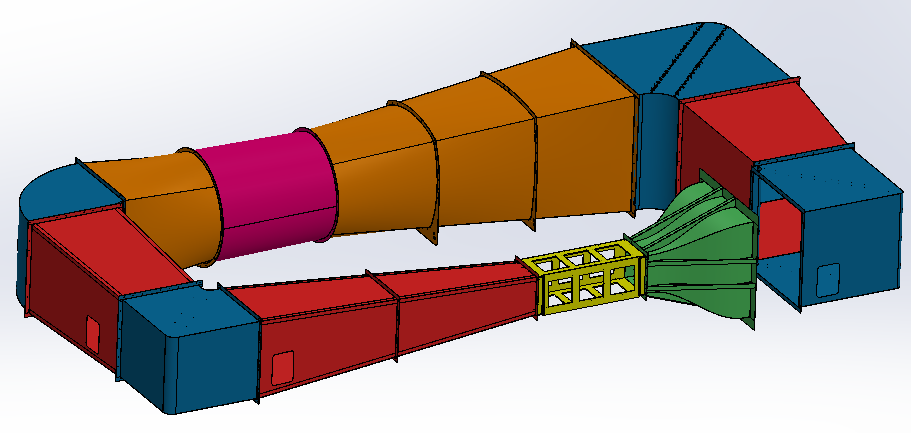
\includegraphics[width=\textwidth]{../photos/whitefield_tunnel.png}
  \put(-360,140){\circled{\Large 1}}
  \put(-415,135){\circled{\Large 2}}
  \put(-440,45){\circled{\Large 3}}
  \put(-395,15){\circled{\Large 4}}
  \put(-320,0){\circled{\Large 5}}
  \put(-250,20){\circled{\Large 6}}
  \put(-180,38){\circled{\Large 7}}
  \put(-132,48){\circled{\Large 8}}
  \put(-80,32){\circled{\Large 9}}
  \put(-60,40){\circled{\Large 10}}
  \put(-25,135){\circled{\Large 11}}
  \put(-50,165){\circled{\Large 12}}
  \put(-180,190){\circled{\Large 13}}
  \put(-315,155){\circled{\Large 14}}
  \caption{CAD model of the University of Notre Dame Whitefield wind-tunnel. The specifications of the tunnel at the numbered cross-sections are shown in Table \ref{tab:03_wind_tunnel_specs}.}
  \label{fig:03_tunnel_model}
\end{figure}
The cross-sectional area and distance from the wind-tunnel fan going upstream are presented in Table \ref{tab:03_wind_tunnel_specs} along with some comments on the segments between some of the cross-sections.
\begin{table}
  \centering
  \caption{Wind-tunnel cross-section specifications}
  \begin{tabular}{c c c l}
    Section & Area (m$^2$) & Z (m) & Comment \\
    \hline \hline
    1 & 5.07 & 0.00 & \multirow{2}{2in}{Circle to Square Transition}\\
    2 & 4.68 & 2.42 & \\
    3 & 4.68 & 4.56 & \\
    4 & 3.57 & 8.65 & \\
    5 & 3.57 & 10.71 & \\
    6 & 1.97 & 14.33 & \multirow{2}{2in}{Cruciform}\\
    7 & 0.84 & 17.99 & \multirow{2}{2in}{Test-Section}\\
    8 & 0.84 & 20.73 & \multirow{2}{2in}{Sixth Order Contraction}\\
    9 & 5.44 & 23.07 & \\
    10 & 5.44 & 24.30 & \\
    11 & 5.44 & 26.54 & \\
    12 & 8.04 & 29.65 & \\
    13 & 8.04 & 31.88 & \multirow{2}{2in}{Circle to Square Transition}\\
    14 & 4.67 & 39.25 & \\
  \end{tabular}
  \label{tab:03_wind_tunnel_specs}
\end{table}
For the distances in Table \ref{tab:03_wind_tunnel_specs} the corners have been straightened out and set to a length equal to the center-line arc from the entrance to the exit of that segment.
The transition segments on either side of the wind-tunnel fan convert the circular cross-section to a square cross-section.
Between cross-section 6 and 7 the diffuser has a cruciform splitting it into four separate segments in which the duct modes were independently marched.
The test-section is 2.75 m long and the main contraction shape from section 8 to 9 follows a fifth-order polynomial.
Acoustic reflections that would be due to turning vanes or other internal structures have been neglected along with the fan hub and motor shaft geometry.

The wind-tunnel was discretized into smaller segments that were a maximum of 0.25 m in length.
The speed throughout the wind-tunnel was determined via isentropic relations and the pressure transmission ratios were computed using Equations \ref{eqn:03_pressure_ratio_with} and \ref{eqn:03_pressure_ratio_against}.
% Redo equation ref
Pressure reflection ratios were calculated using Equations \ref{eqn:03_pressure_ratio_with_reflected} and \ref{eqn:03_pressure_ratio_against_reflected} and verified to be small.
Figure \ref{fig:03_tunnel_discretization} shows these parameters for the tunnel at a Mach number of 0.6 in the test-section with flow going from right-to-left.
\begin{figure}
  \centering
  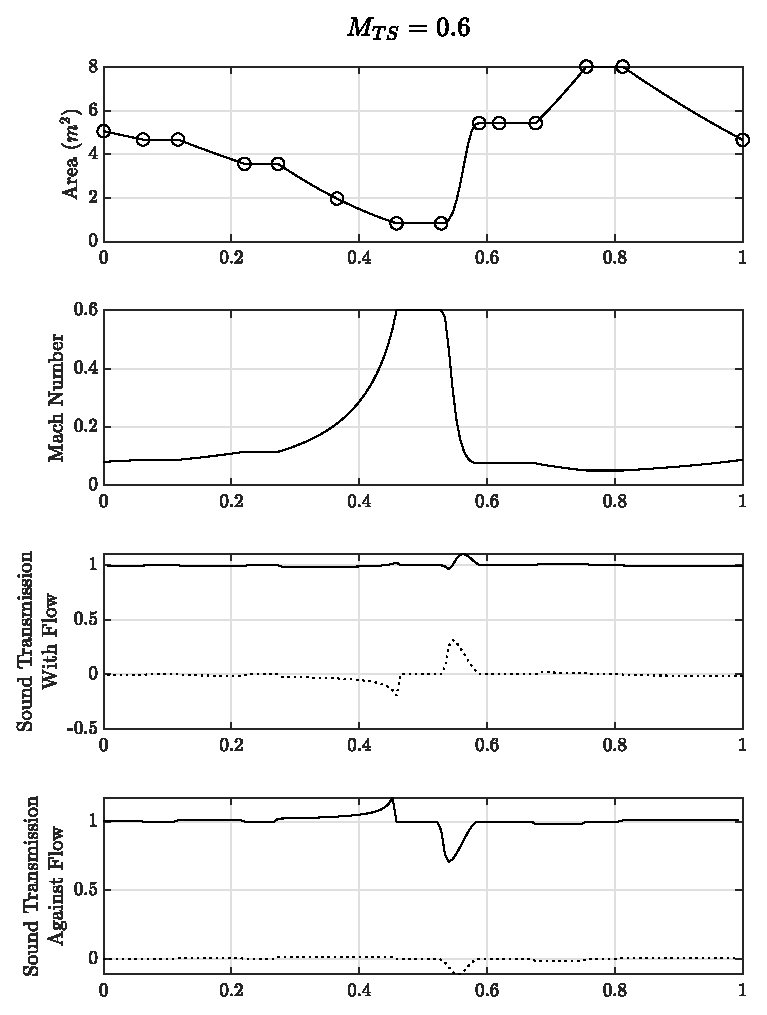
\includegraphics{../matlab/03_aero_optics_acoustics/tunnel_discretization_0.60.eps}
  \put(-162,375){\rotatebox{90}{\large Test Section}}
  \put(-215,60){\large Acoustic Propagation $\Longrightarrow$}
  \put(-235,190){\large $\Longleftarrow$ Acoustic Propagation}
  \caption{Wind-tunnel discretization at a Mach number of 0.6. The solid lines in the sound transmission plots represent the transmitted pressure ratio while the dotted lines represent the reflected pressure ratio.}
  \label{fig:03_tunnel_discretization}
\end{figure}
For most of the wind-tunnel the Mach number is around 0.1 with the transmission pressure ratio (solid lines) at effectively unity.
In the regions of rapid Mach number change around the contraction and the test-section diffuser, the transmission pressure ratio can deviated significantly from unity, especially for sound waves traveling upstream.
These regions also show some reflected pressure ratios (dotted lines) that are non-negligible.
For acoustic waves traveling in both directions, the section on the opposite side of the test section produces some reflected acoustic waves back into the test section.

The wind-tunnel fan was modeled using a circular duct mode of $m=8$ and $n=0$ at a frequency of 520 Hz which corresponds to the blade-passing frequency of the Mach number 0.6 case.
The duct mode of $m=8$ and $n=0$ is the largest cut-on mode in which the azimuthal mode number is a whole-number fraction of the total number of fan blades, 32.
The peak-to-peak acoustic pressure of the fan was set to unity to allow the results to be easily scaled.
To check for the possibility of some duct modes only being present at certain orientations of the fan blades, the initial acoustic pressure disturbance was rotated by replacing $\omega t$ in the temporal portion of Equation \ref{eqn:02_pressure_solution_duct} with a phase offset that varied from 0 to 2$\pi$.

Cross-sectional slices of the acoustic field as the waves march upstream from the fan through the circle to square transition are shown in Figure \ref{fig:03_transition_acoustics}.
\begin{figure}
  \centering
  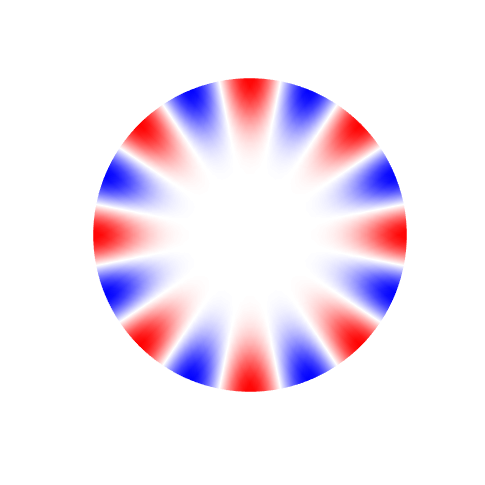
\includegraphics[trim={0.3in 0.3in 0.3in 0.3in},clip]{../matlab/03_aero_optics_acoustics/tunnel_slices/tunnel_acoustic_against_0.6_8_0_0_001.eps}
  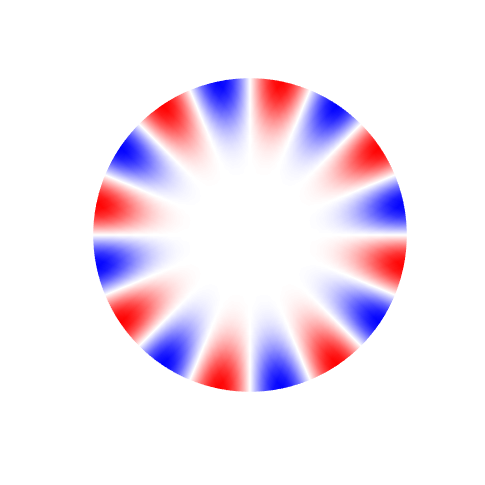
\includegraphics[trim={0.3in 0.3in 0.3in 0.3in},clip]{../matlab/03_aero_optics_acoustics/tunnel_slices/tunnel_acoustic_against_0.6_8_0_1.5708_001.eps} \\
  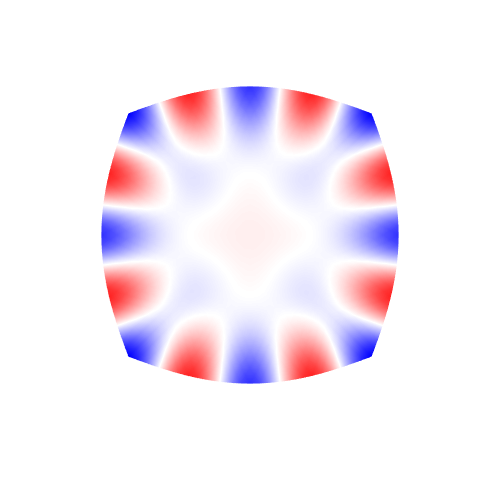
\includegraphics[trim={0.3in 0.3in 0.3in 0.3in},clip]{../matlab/03_aero_optics_acoustics/tunnel_slices/tunnel_acoustic_against_0.6_8_0_0_006.eps}
  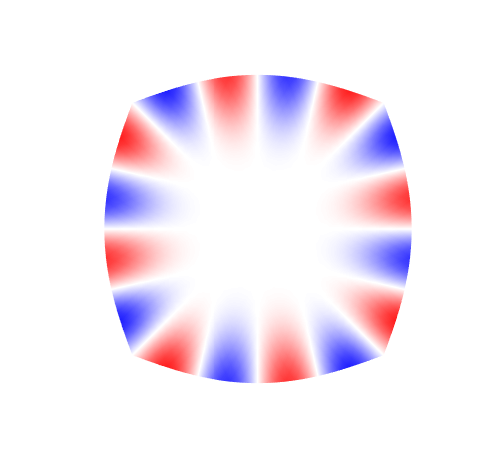
\includegraphics[trim={0.3in 0.3in 0.3in 0.3in},clip]{../matlab/03_aero_optics_acoustics/tunnel_slices/tunnel_acoustic_against_0.6_8_0_1.5708_006.eps} \\
  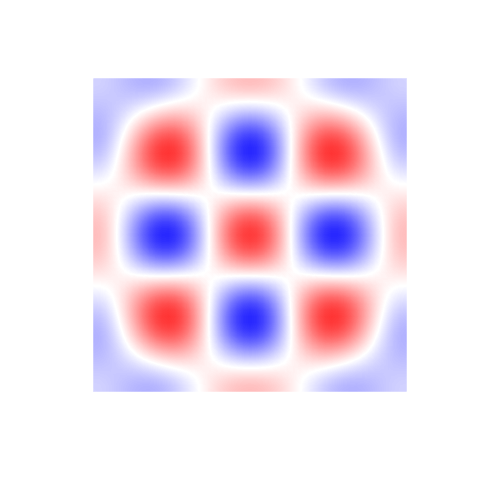
\includegraphics[trim={0.3in 0.3in 0.3in 0.3in},clip]{../matlab/03_aero_optics_acoustics/tunnel_slices/tunnel_acoustic_against_0.6_8_0_0_012.eps}
  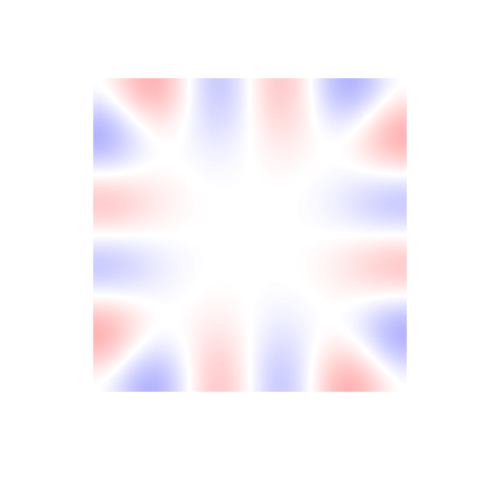
\includegraphics[trim={0.3in 0.3in 0.3in 0.3in},clip]{../matlab/03_aero_optics_acoustics/tunnel_slices/tunnel_acoustic_against_0.6_8_0_1.5708_012.eps}
  \caption{Cross-sectional slices of the acoustic field through the circle to square transition for the acoustic waves traveling upstream. Left side are the waves traveling from the fan at a phase of 0 radians and the right side at a phase of $\pi$/2 radians. The top plots are the fan acoustic field, the middle plots are halfway through the transition, and the bottom plots are just into the square duct.}
  \label{fig:03_transition_acoustics}
\end{figure}
The plots on the left side are at an initial phase angle of 0 radians and the right side are at a phase angle of $\pi$/2 radians.
The top plots are the cross-sectional slices of the acoustic field directly upstream of the fan, the middle plots are halfway through the transition, and the bottom plots are just into the square duct.
As an acoustic wave propagates upstream, a phase shift can be observed with the halfway transitioned cross-sectional slices having an opposite local phase.
As the acoustic wave enters the square duct the 0 radian phase, left side, bears little resemblance to the original acoustic wave while the $\pi$/2 radian phase shows some significant similarities.

The acoustic field cross-section at the center of the test-section is shown in Figure \ref{fig:03_test_section_acoustics} for a variety of initial phase angles.
\begin{figure}
  \centering
  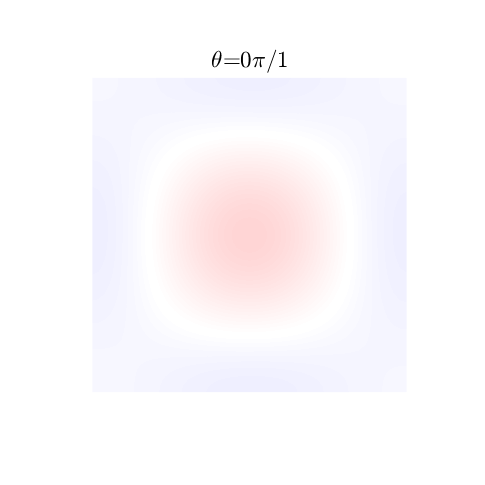
\includegraphics[trim={0.3in 0.3in 0.3in 0.2in},clip]{../matlab/03_aero_optics_acoustics/tunnel_slices/tunnel_acoustic_against_0.6_8_0_0_081.eps}
  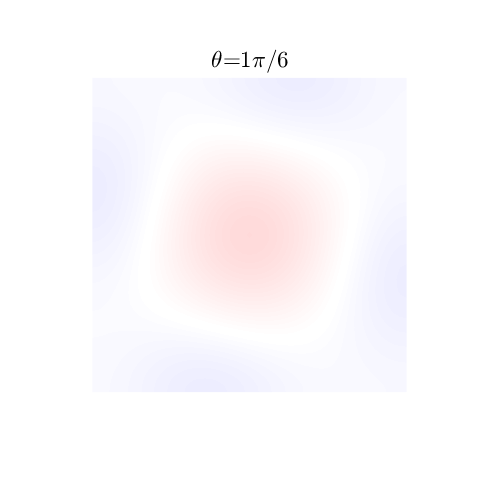
\includegraphics[trim={0.3in 0.3in 0.3in 0.2in},clip]{../matlab/03_aero_optics_acoustics/tunnel_slices/tunnel_acoustic_against_0.6_8_0_0.5236_081.eps}
  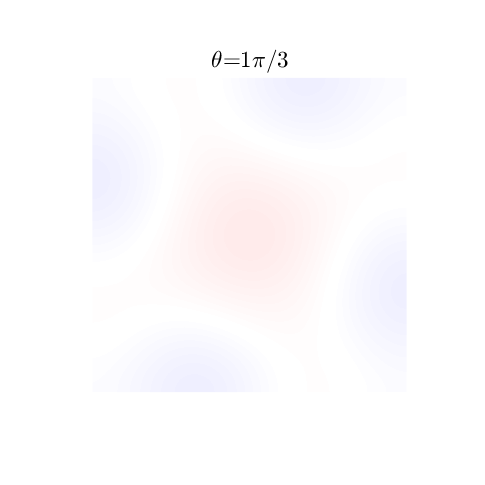
\includegraphics[trim={0.3in 0.3in 0.3in 0.2in},clip]{../matlab/03_aero_optics_acoustics/tunnel_slices/tunnel_acoustic_against_0.6_8_0_1.0472_081.eps}
  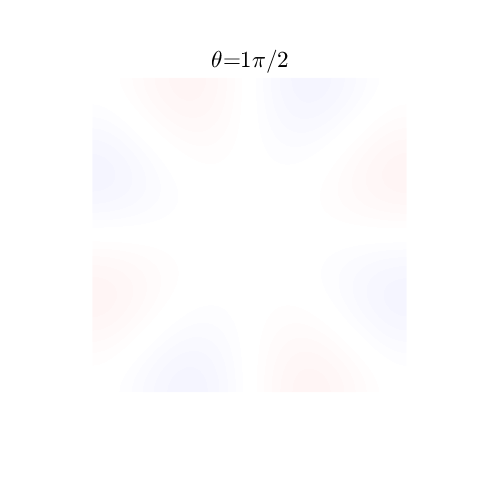
\includegraphics[trim={0.3in 0.3in 0.3in 0.2in},clip]{../matlab/03_aero_optics_acoustics/tunnel_slices/tunnel_acoustic_against_0.6_8_0_1.5708_081.eps}
  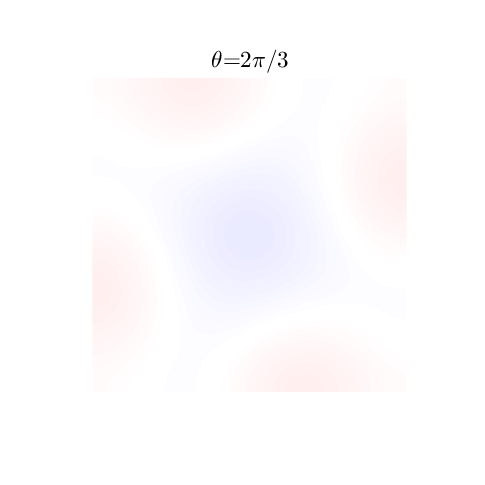
\includegraphics[trim={0.3in 0.3in 0.3in 0.2in},clip]{../matlab/03_aero_optics_acoustics/tunnel_slices/tunnel_acoustic_against_0.6_8_0_2.0944_081.eps}
  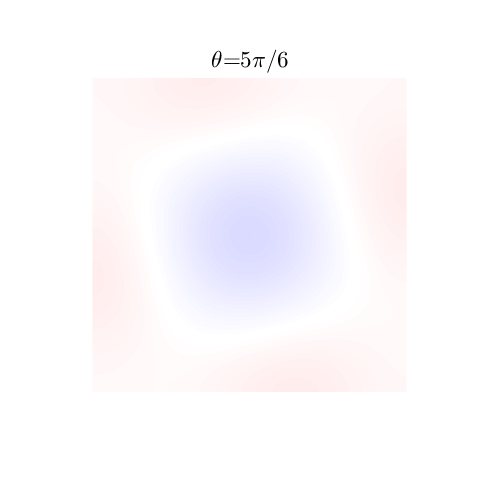
\includegraphics[trim={0.3in 0.3in 0.3in 0.2in},clip]{../matlab/03_aero_optics_acoustics/tunnel_slices/tunnel_acoustic_against_0.6_8_0_2.618_081.eps}
  \caption{Cross-sectional acoustic field slices in the center of the test-section at various initial phase angles.}
  \label{fig:03_test_section_acoustics}
\end{figure}
As the fan blades rotate, so to does the acoustic field within the test-section.
The real component of the duct modes are shown in Figure \ref{fig:03_test_section_modes} as a function of the initial phase angle.
The primary duct mode in the test-section is the $m=2$, $n=2$ mode with contributions from pairs of modes $m=0,2$, $n=2,0$ which are in phase with one another and out of phase mode pairs $m=1,3$, $n=3,1$.
Note that for Figures \ref{fig:03_test_section_modes} and \ref{fig:03_test_section_modes_with} the $m=0,2$, $n=2,0$ modes overlap one another in the plots.
\begin{figure}
  \centering
  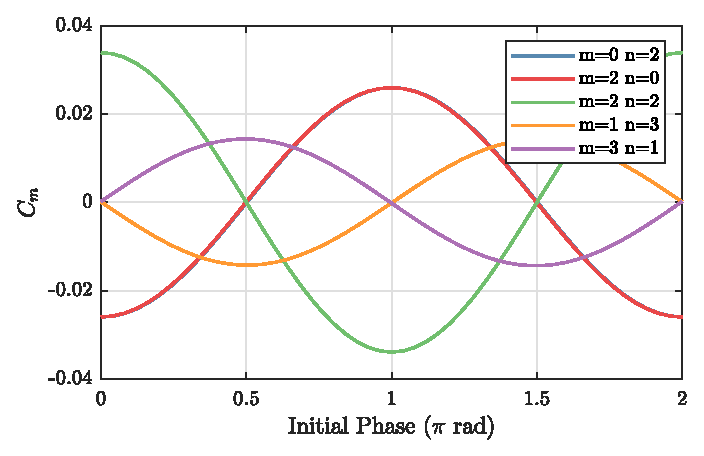
\includegraphics{../matlab/03_aero_optics_acoustics/tunnel_acoustic_against_0.6_8_0.eps}
  \caption{The real component of the acoustic mode coefficients making up the upstream-traveling acoustic field in the middle of the test-section as a function of the initial phase angle.}
  \label{fig:03_test_section_modes}
\end{figure}
These five modes can be used to simulate the optical response of the fan driven acoustics inside of the test section by using the maximum value of the modal coefficient and a relative phase angle between the different modes by using Equation \ref{eqn:02_pressure_solution_duct} and
\begin{equation}
  \widehat{\opd}(x,y) = \frac{K_{GD}}{c_0^2}\int_{z_1}^{z_2} \hat{p}(x,y,z)_{Ap}dz \textrm{,}
  \label{eqn:03_opd_complex}
\end{equation}
where $\widehat{\opd}$ is the complex optical path difference and $K_{GD}$ is the Gladstone-Dale constant.
The temporal portion of Equation \ref{eqn:02_pressure_solution_duct} can be applied after the integration process in Equation \ref{eqn:03_opd_complex} and just before taking the real component to simulate a measured value at a particular instant in time.

The acoustic duct modes in the center of the test-section for the acoustic waves traveling in the direction of the flow are shown in Figure \ref{fig:03_test_section_modes_with}.
\begin{figure}
  \centering
  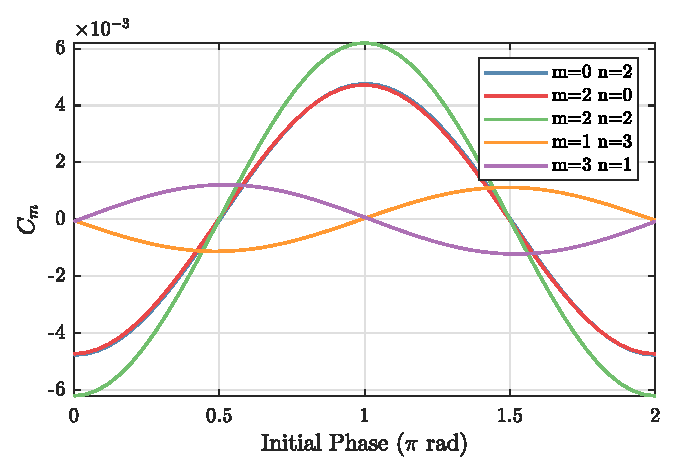
\includegraphics{../matlab/03_aero_optics_acoustics/tunnel_acoustic_with_0.6_8_0.eps}
  \caption{The real component of the acoustic mode coefficients making up the downstream-traveling acoustic field in the middle of the test-section as a function of the initial phase angle.}
  \label{fig:03_test_section_modes_with}
\end{figure}
The downstream-traveling acoustic field inside of the test-section is comprised of the same duct modes as the upstream-traveling acoustic field but the mode coefficient are approximately an order-of-magnitude lower.
All of the phase offsets for the modes remain the same except for the $m=2$, $n=2$ mode which is now different by $\pi$ radians compared to the upstream-traveling modes in Figure \ref{fig:03_test_section_modes}.
When the downstream-traveling acoustic field enters the cruciform after the test-section a portion of it is reflected, see Figure \ref{fig:03_tunnel_discretization}.
When the maximum reflected pressure ratio, approximately -0.2, is combined with the strength of the downstream-traveling acoustic field, the acoustic field reflected back into the test-section is 1-2 orders-of-magnitude lower than the upstream-traveling acoustic field from the fan.
On the other hand, the reflected field from the upstream-traveling acoustic field after it leaves the test-section is on the same order-of-magnitude as the downstream-traveling acoustic field.

A comparison between a measured optical wavefront that has been band-pass filtered at the blade-passing frequency and a simulated optical wavefront that has been shot through the estimated acoustic field computed by the mode-marching method is shown in Figure \ref{fig:03_tunnel_comparison}.
\begin{figure}
  \centering
  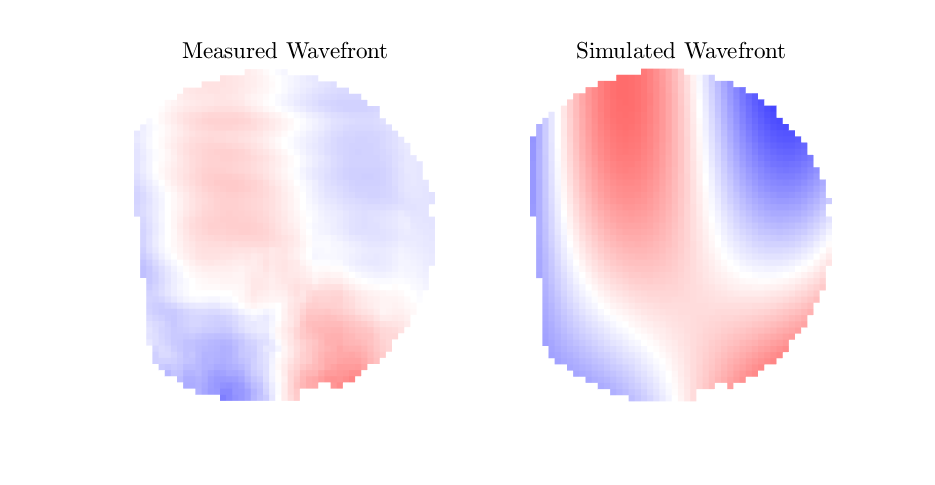
\includegraphics{../matlab/03_aero_optics_acoustics/tunnel_comparison.eps}
  \caption{Comparison of a measured optical wavefront and a simulated one passing through the estimated acoustic field.}
  \label{fig:03_tunnel_comparison}
\end{figure}
Qualitatively, there is significant agreement between the two wavefronts.
Since there was no microphones installed in either the test-section or around the wind-tunnel fan, there cannot be a quantitative comparison made.

\section{Summary}
\label{sect:03_summary}
Acoustic waves affect the transmission of light by causing the local index-of-refraction to change with the pressure fluctuations.
When the acoustic field is well modeled, as was the case with the spherical wave measurements, an optical wavefront measurement can provide an accurate measurement of the acoustic field strength non-intrusively.

The mode-marching method provides a computationally rapid way of estimating an acoustic signal as it travels through a duct system like a wind-tunnel.
This method assumes that the reflected component will be minimal and can be ignored.
A significant contribution of this work to the computational procedure of this method is computing the eigen-functions for the wind-tunnel fan transition geometries that are neither circular nor rectangular.
These computations would become even more costly if the cross-section cannot be assumed to have a uniform flow speed \cite{Wilson-2019-VV2zh7Au}.
Finally, note that the mode-marching method used here has neglected the effect that the corners would have on the signal or other internal geometry such as the turning vanes or the turbulence screens.

The main benefit to using a mode-marching method is to simulate narrow-band signals that appear in the optical wavefront spectra and to have some level of confidence that the source of that signal is the wind-tunnel fan.
If the narrow-band signal does not match up with the simulated signal, it could have a source that may not be due to the testing environment and would likely need to be investigated further.
If there is significant agreement between the measured and simulated signals, a simple stop-band filter could be used to eliminate the contamination.
